\documentclass[11pt]{article}

\usepackage[letterpaper,margin=0.75in]{geometry}
\usepackage{booktabs}
\usepackage{caption}
\usepackage{graphicx}
\usepackage{listings}
\usepackage{float}
\usepackage{scrextend}
\usepackage{hyperref}
\usepackage[parfill]{parskip}
\renewcommand{\lstlistingname}{Snippet}


\begin{document}

\lstset{
  language=Python,
  basicstyle=\small,          % print whole listing small
  keywordstyle=\bfseries,
  identifierstyle=,           % nothing happens
  commentstyle=,              % white comments
  stringstyle=\ttfamily,      % typewriter type for strings
  showstringspaces=false,     % no special string spaces
  numbers=left,
  numberstyle=\tiny,
  numbersep=5pt,
  frame=tb,
}

\title{Reliable Transport}

\author{Brandt Elison & Joe Eklund}

\date{February 20, 2016}

\maketitle

\section{Implementation}

Our implementation of TCP reliability was a modification of the \href{https://github.com/zappala/bene/}{bene network simulator}. However, before we began writing any code to implement reliability we drew a diagram outlining the steps required to implement TCP. Figure \ref{diagram1} is a digitized version of this outline.

The following numbers correspond to the step numbers shown in Figure \ref{diagram1} and in which method(s) they were implemented. These methods can be found in tcp.py in the source code.

\begin{enumerate}
  \item TCP Constructor
  \item \texttt{send(data)}
  \item \texttt{send\textunderscore max()}
  \item \texttt{send\textunderscore packet(data, sequence)}
  \item \texttt{handle\textunderscore ack(packet), cancel\textunderscore timer()}
  \item \texttt{handle\textunderscore ack(packet)}
  \item \texttt{adjust\textunderscore timeout(sample\textunderscore rtt)}
  \item \texttt{send\textunderscore packet(data, sequence), send\textunderscore max()}
  \item \texttt{retransmit(event)}
  \item \texttt{retransmit(event)}
  \item \texttt{retransmit(event)}
  \item \texttt{send\textunderscore packet(data, sequence)}
  \item \texttt{send\textunderscore packet(data, sequence), send\textunderscore max()}
  \item \texttt{send\textunderscore max()}
  \item[R1.] \texttt{handle\textunderscore data(packet)}
  \item[R2.] \texttt{send\textunderscore ack(time\textunderscore stamp)}
\end{enumerate}


\begin{figure}[H]
\caption{The diagram of our reliability outline.}
\label{diagram1}
  \centering
  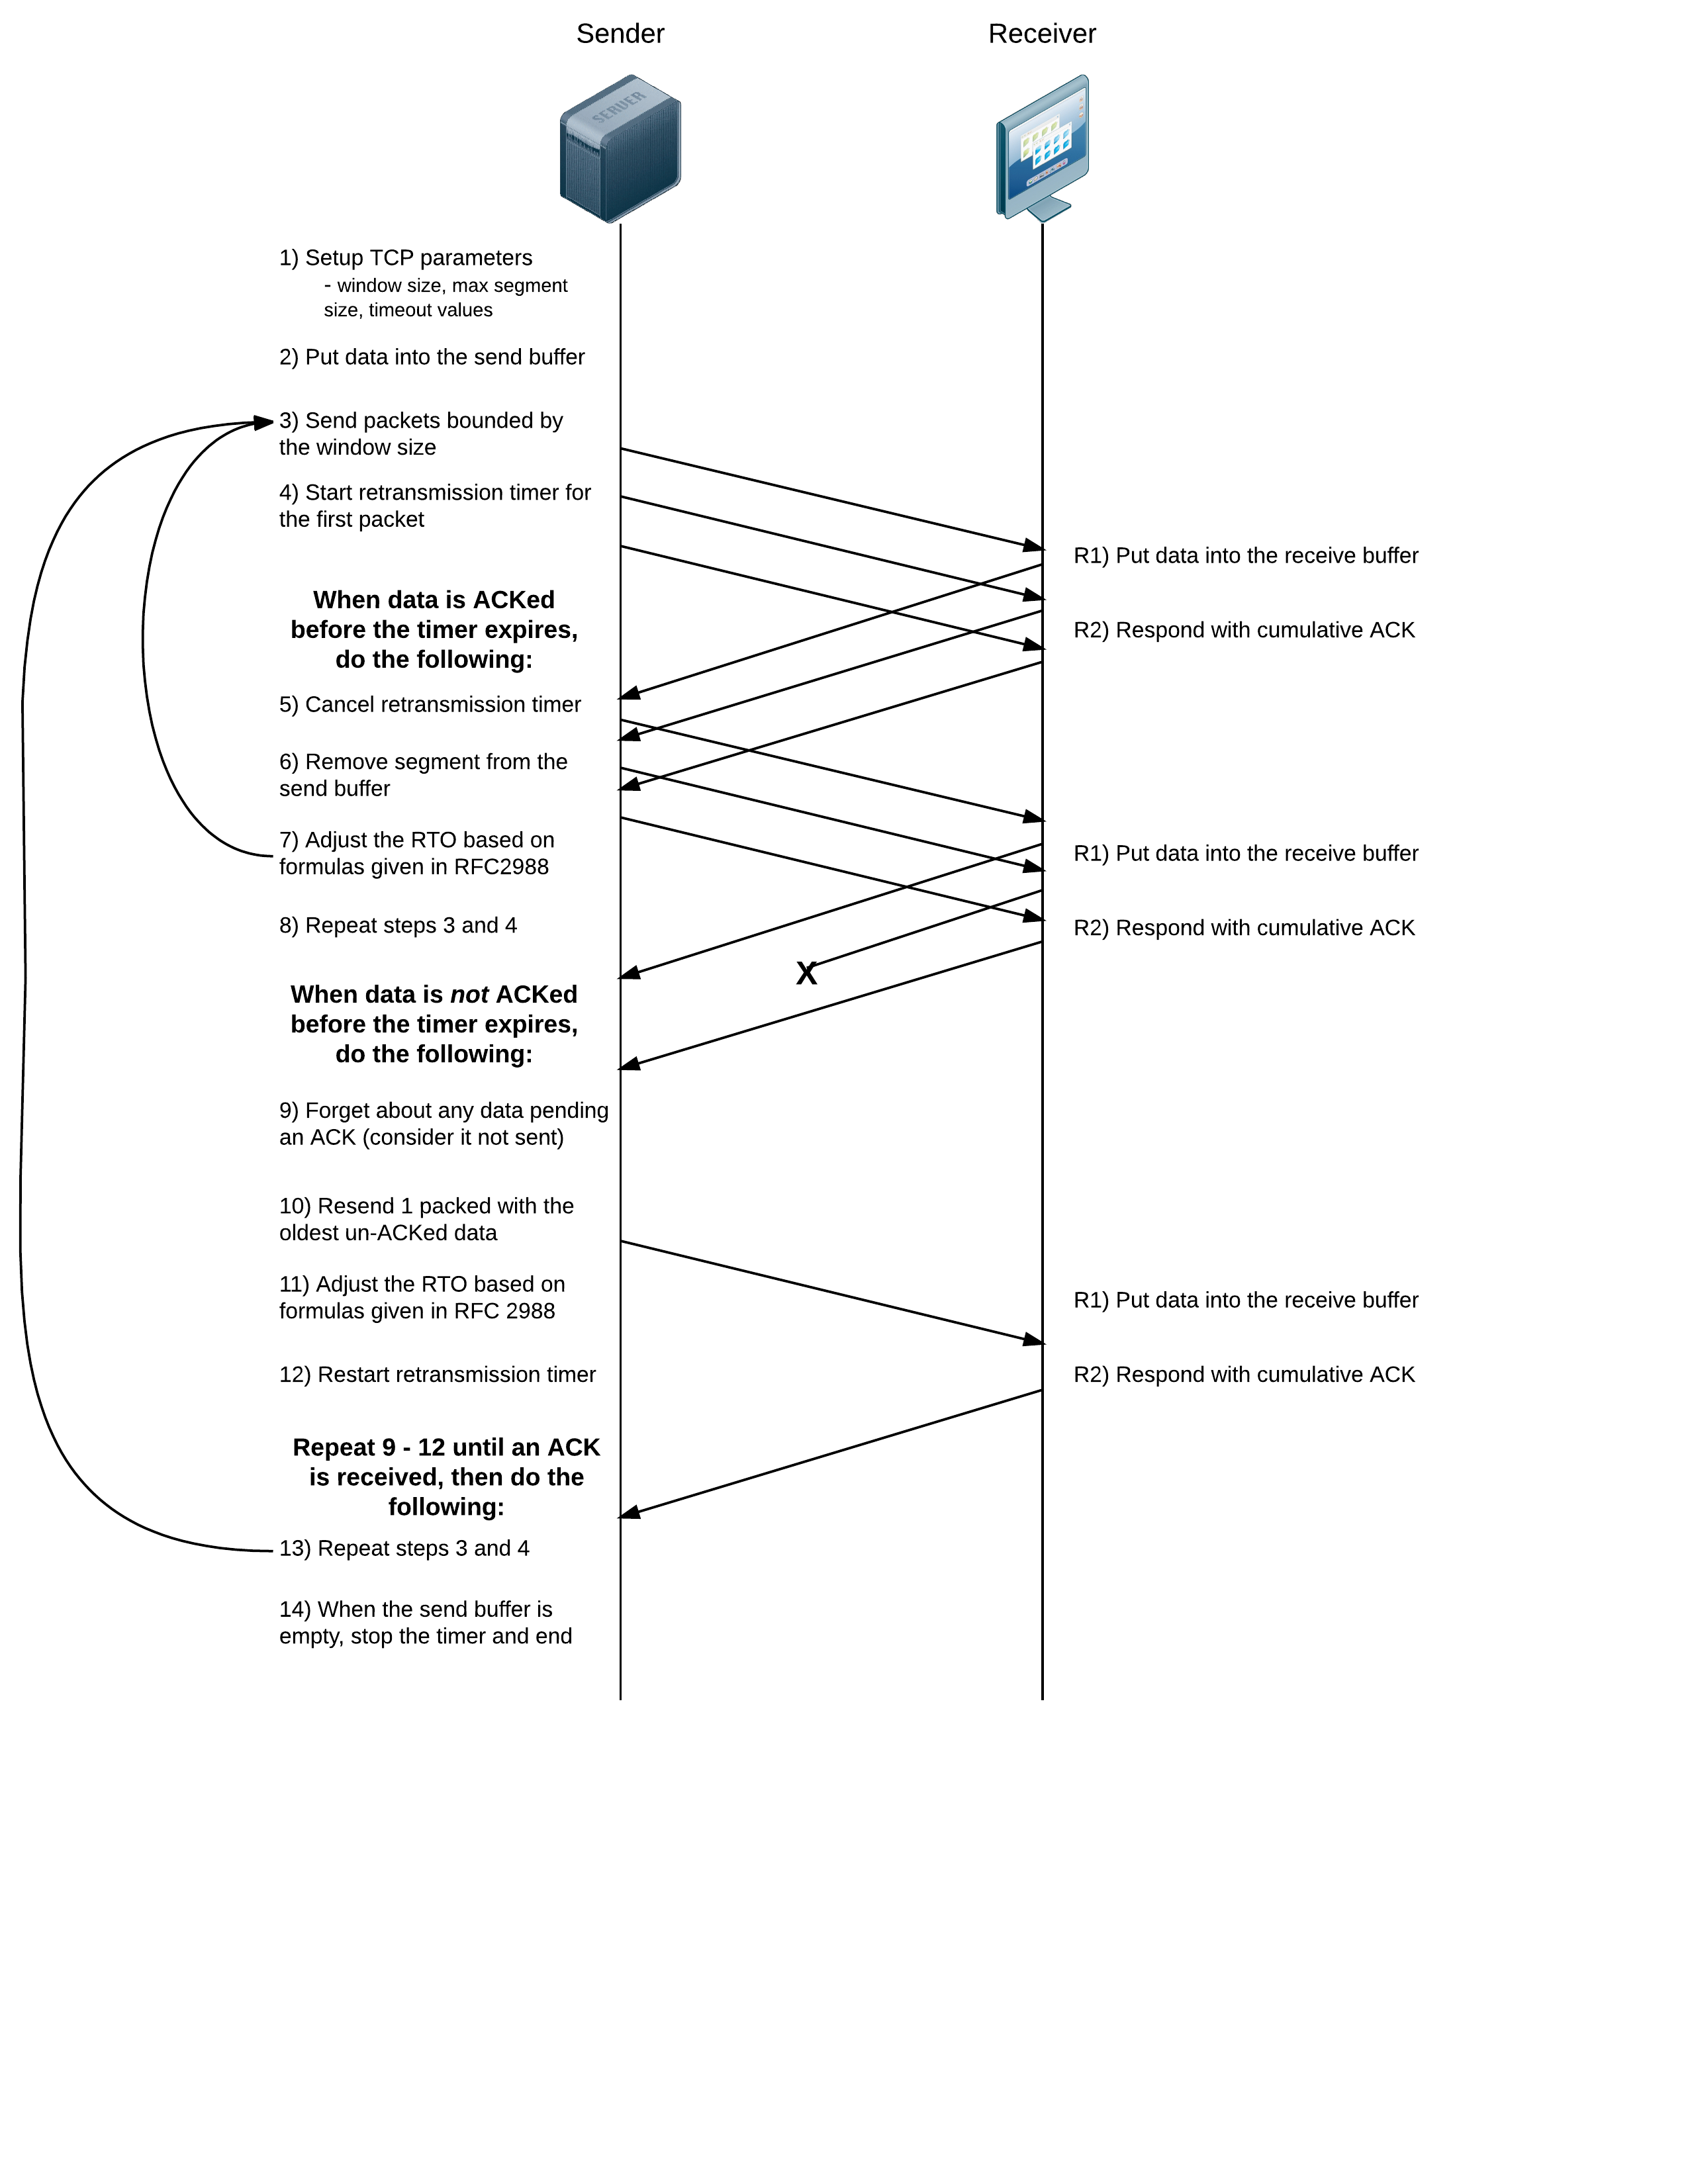
\includegraphics{diagram1}
\end{figure}

We added a dynamic retransmission timer that uses an exponetial weighted moving average (EWMA) for the timer value and the variance. We implemented our dynamic timer in tcp.py by creating a function called \texttt{adjust\textunderscore timeout(sample\textunderscore rtt)} which is invoked every time the sender receives an ACK for un-ACKed data. We also modified \texttt{retransmit()} to double the timeout value when the function is invoked. This is in keeping with \href{http://www.ietf.org/rfc/rfc2988.txt}{RFC 2988}.

\section{Test Results}

After implementing reliable transport, we ran tests on two files called test.txt and internet-architecture.pdf. We wrote a script that copies the test files from one directory to another and then diffs them to verify that our implementation of TCP reliability functions correctly. 

For each file we tested loss rates ranging from 0.0 to 0.5 on both a fixed one second timer and dynamic retransmission timer. The dynamic timer uses an EWMA for the timer value and variance. For test.txt we recorded the average time it took to transfer the file over 1000 tests. For internet-architecture.pdf we averaged tranfer times over 100 tests. The results of these tests are shown in tables \ref{tbltest} and \ref{tblinternet} respectively.

\begin{table}[H]
\begin{center}
\caption{Test results for transfering test.txt}
\label{tbltest}
\begin{tabular}{ccc}
  \toprule
  Loss Rate & Fixed Timer (sec) & Dynamic Timer (sec) \\
  \midrule
  0.0 & 0.0832 & 0.0832 \\
  0.1 & 1.175 & 1.677 \\
  0.2 & 2.312 & 7.735 \\
  0.5 & 16.078 & 2,067,467.769 \\
  \bottomrule
\end{tabular}
\end{center}
\end{table}

\begin{table}[H]
\begin{center}
\caption{Test results for transfering internet-architecture.pdf}
\label{tblinternet}
\begin{tabular}{ccc}
  \toprule
  Loss Rate & Fixed Timer (sec) & Dynamic Timer (sec) \\
  \midrule
  0.0 & 1.084 & 1.084 \\
  0.1 & 37.0 & 48.093 \\
  0.2 & 71.484 & 162.994 \\
  0.5 & 389.159 & 391,497,109.508 \\
  \bottomrule
\end{tabular}
\end{center}
\end{table}

Snippet \ref{retransOutput} shows trace output for the state of the dynamic retransmission timer while transmitting test.txt with a loss rate of 0.1.

\begin{lstlisting}[caption={Dynamic retransmission output},label=retransOutput]
Starting timer with timeout of: 3.0
Received ACK with RTT of: 0.0208
Timeout adjusted from 3.0 to 1.0208
Starting timer with timeout of: 1.0208
Received ACK with RTT of: 0.0216
Timeout adjusted from 1.0208 to 1.0209
Starting timer with timeout of: 1.0209
**Timer expired. Doubled timeout to 2.0418
Starting timer with timeout of: 2.0418
Received ACK with RTT of: 0.0208
Timeout adjusted from 2.0418 to 1.0208875
Starting timer with timeout of: 1.0208875
Received ACK with RTT of: 0.0216
Timeout adjusted from 1.0208875 to 1.0209765625
Starting timer with timeout of: 1.0209765625
Received ACK with RTT of: 0.0224
Timeout adjusted from 1.0209765625 to 1.02115449219
Received ACK with RTT of: 0.0216
Timeout adjusted from 1.02115449219 to 1.02121018066
\end{lstlisting}

As evidenced from Snippet \ref{retransOutput}, the timeout converges from 3.0 seconds to about 1.02 seconds. This shows that the dynamic retransmission timer is in fact converging to the right value over time. Lines 7 and 8 of Snippet \ref{retransOutput} show that exponential backoff works as expected.

Tables \ref{tbltest} and \ref{tblinternet} show that with a loss rate of 0.0, both the fixed timer and dynamic timer transmit files in the same amount of time. This makes sense because we never have to retransmit packets and the timer never expires. The transmission times are relatively short from the 0.0 to 0.2 loss rate range for both types of timers. However, the time it takes to transmit with a dynamic timer of a loss rate of 0.5 is untenable; the transmission of internet-architecture.pdf took 391,497,109.508 seconds (12.41 years) which is clearly unacceptable.

\section{Experiments}

Our experiments consisted of sending the file internet-architecture.pdf on a network with the following parameters:

\begin{itemize}
\item Link speed $n_1$ to $n_2$: 10 Mbps
\item Link speed $n_2$ to $n_3$: 10 Mbps
\item Propagation delay $n_1$ to $n_2$: 10 ms
\item Propagation delay $n_2$ to $n_3$: 10 ms
\item Queue Size: 100 Packets
\item Loss Rate: 0.0
\end{itemize}

We ran 6 tests, changing the window size each time in the range of 1,000 to 20,000 bytes (see Table \ref{tblexper} Column 1 for the exact window sizes we used). Figures \ref{throughput} and \ref{queueing} respectively plot the Throughtput and Queueing Delay columns of Table \ref{tblexper} vs each of the window sizes in Table \ref{tblexper}.

\begin{table}[H]
\begin{center}
\caption{Test results for transfering internet-architecture.pdf}
\label{tblexper}
\begin{tabular}{llll}
  \toprule
  Window Size (bytes) & Transmission Time (sec) & Throughput (bits/sec) & Average Queueing Delay (ms) \\
  \midrule
  1,000 & 10.711 & 384,270.68 & 0.0 \\
  2,000 & 05.366 & 767,079.34 & 0.001553 \\
  5,000 & 02.145 & 1,918,762.49 & 0.01553 \\
  10,000 & 01.084 & 3,795,738.90 & 0.06990 \\
  15,000 & 00.731 & 5,632,279.53 & 0.1631 \\
  20,000 & 00.552 & 7,462,002.55 & 0.2951 \\
  \bottomrule
\end{tabular}
\end{center}
\end{table}

\begin{figure}[H]
\caption{Window Size vs Throughput for transmitting internet-architecture.pdf}
\label{throughput}
  \centering
  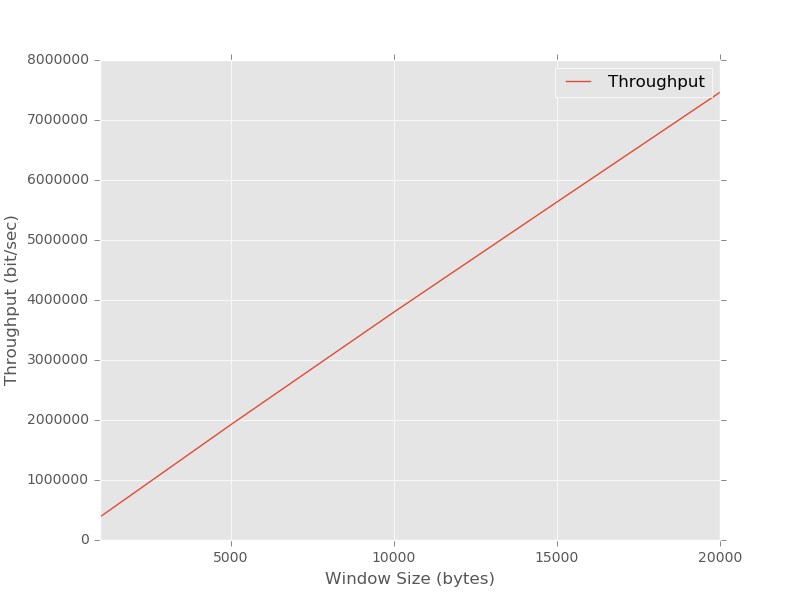
\includegraphics[width=15cm]{throughput}
\end{figure}

By looking at Figure \ref{throughput} we can see our throughput varies linearly with our window size. This makes sense because elements that would usually prevent this linear relationship, such as packet loss or low bandwidth on the link, are not factors in this situation. Our loss rate was set to 0.0, so there was no simulated packet loss to reduce throughput; our link speed was 10 Mbps, which gives plenty of bandwidth to handle the window size of 20 kB. Therefore, doubling the window size does simply double the rate at which the receiver gets data a.k.a. doubles the throughput.

\begin{figure}[H]
\caption{Window Size vs Queueing Delay for transmitting internet-architecture.pdf}
\label{queueing}
  \centering
  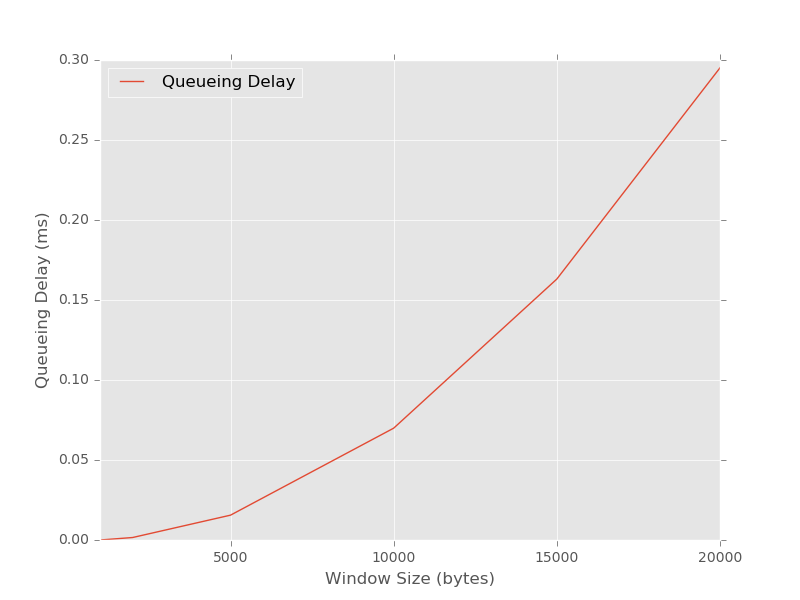
\includegraphics[width=15cm]{queueing}
\end{figure}

By looking at Figure \ref{queueing} we can see our average queueing delay looks like it varies exponentially with window size. Again this result makes sense because the queueing delay builds slowly at first while the link is able to handle the volume of packets, but as the window size gets larger, the link will have to queue more of the packets until all of the aditional packets are queued.

While the exponential increase makes the queueing delay seem substantial, it should be remembered that the unit of measurement in Figure \ref{queueing} for queueing delay is milliseconds. Even though the queueing delay looks large for a window size of 20,000 bytes, the delay is actually only 0.2951 ms per packet. This is because our link is so fast and our loss rate is 0.0.

\end{document}
